\documentclass[pdf]
{beamer}
\mode<presentation>{}
%% preamble
\title{Model inference from protein time-course in Hematopoietic Stem Cells (HSC)}
\subtitle{}
\author[shortname]{Pandu Raharja \inst{1, 2} \and Rene Schoeffel \inst{1, 2} \and Michael Strasser \inst{3}}
\institute[shortinst]{\inst{1} Technische Universit\"at M\"unchen \and %
                      \inst{2} Ludwig-Maximilians-Universit\"at M\"unchen \and %
                      \inst{2} Institute of Computational Biology (ICB), Helmholtz Zentrum M\"unchen}
\begin{document}

%% title frame
\begin{frame}
\titlepage
\end{frame}

%% normal frame
\begin{frame}{Introduction}
	\begin{itemize}
		\item Dynamics of hematopoetic stem cell maturation cell from Common Myeloid Progenitor (CMP) to Megakaryocyte-Erythroid Progenitor (MEP) and Granulocyte-Macrophage Progenitor (GMP)
	\end{itemize}
	
	\begin{figure}[ht]
		\begin{center}
			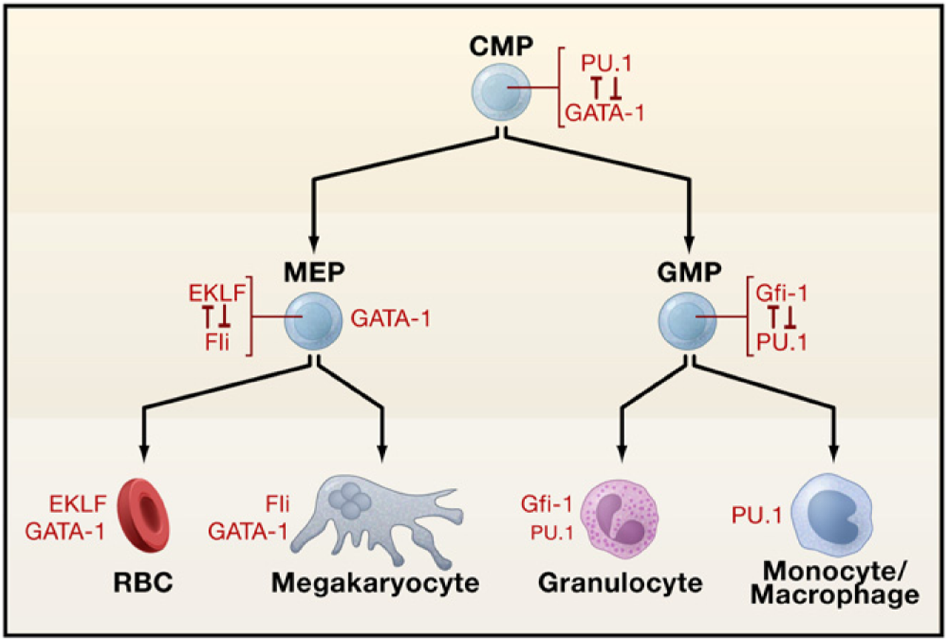
\includegraphics[height=2in]{figures/homatopoietic_focus.png}
			~\footnote{Graf \& Enver, \textit{Nature}, 2009}
		\end{center}
	\end{figure}
\end{frame}

\begin{frame}{Introduction (cont'd)}
	\begin{itemize}
	\item MEP and GMP yield not 50\% : 50\% as previously thought, but 70\% : 30\%
	\item Assumed dynamics between \texttt{Pu.1} and \texttt{Gata1} in cell maturation fate
	\begin{itemize}
		\item Dynamics assumed to be a bistable toggle-switch system
	\end{itemize}
	\end{itemize}
\end{frame}

\begin{frame}{Problems}
	\begin{itemize}
	\item Stochaticity in single cell is more punctuatedy
	\end{itemize}
\end{frame}



\end{document}